% \documentclass[portrait,25pt]{sciposter}
\documentclass[]{beamer}
\usepackage[orientation=portrait,size=a0extended,scale=1,debug]{beamerposter}
\usepackage[utf8x]{inputenc}
%\usepackage[spanish]{babel}
\usepackage{amsmath}
\usepackage{amsfonts}
\usepackage{amssymb}
\usepackage{wasysym}
\usepackage{graphicx}
\usepackage{eurosym}
\usepackage{multicol}
\usepackage{fancyhdr}
\usepackage{tikz}
\usepackage{colortbl}
\usepackage[version=3]{mhchem}
\usepackage[lf]{venturis}

\setbeamertemplate{caption}[numbered] 

%\event{VII Congreso de Investigadores en Formaci\'on -- Universidad de C\'ordoba}
\date{Royal Statistical Society International Conference 2021\\
Manchester (6-9 September 2021)}
\title{Computational Methods for Modelling Mortality and Fertility Projections: Application to Spanish Demography}
\author{Jos\'e Rafael Caro-Barrera\textsuperscript{1,
\includegraphics[height=0.75em]{orcid.png}}}
\institute{\textsuperscript{1} Dept. of Statistics, Econometrics, Operational Research and Applied Economics\\ University of C\'ordoba -- Spain}


%%%%%%%%%%%%%%%%%%%%
% Document started %
%%%%%%%%%%%%%%%%%%%%

\mode<presentation>{
\usetheme{Regensburg}
\usecolortheme{PhysikPoster3} %PhysikPoster for green, PhysikPoster2 for darkblue, PhysikPoster3 for blue
}

\begin{document}
\begin{frame}{\vspace{1ex}\hfill Keywords: \bfseries \textit{Demography, Longevity, Stochastic Mortality Modelling, Bayesian Fertility Models.}}
	\begin{columns}[t]
	\column{.45\columnwidth}

\vspace{-1.5cm}
%%%%%%%%%%%%%%%% RESUMEN (ABSTRACT)%%%%%%%%%%%%%%%%%
\begin{block}{Abstract}
			\vspace{-0.5cm}%\small
			%\begin{multicols}{2}
				\setbeamertemplate{bibliography item}[text]
				\bibliographystyle{unsrt}
				\bibliography{literature}
				Spain faces a demographic future with low birth rates. In addition, it is one of the countries with a higher life expectancy, therefore, for economic, social and politics purposes is important to project and forecast such mortality and fertility rates. Mortality and fertility rates are simulated for this country using GAPC stochastic models for mortality forecasting and a Bayesian projection model for fertility projections.
			%\end{multicols}
		\end{block}
		
		\vspace{-0.5cm}  %%%%%%%%%%%%%%%%%%%%%%%%%%%%%%%%%%%%%%%%%%%%%%%	
		\begin{block}{Structure and Methodology}
			\setlength{\parindent}{1.2em}
			\setlength{\parskip}{0.5ex}
			First section points out the worldwide demographical transition and the expected rates for longevity and fertility phenomena for next years. Second and third sections are devoted to fit and simulate mortality and fertility rates for Spain using models and computational methods with \textbf{R}. Finally, main conclusions are addressed and most relevant references are provided. 
		\end{block}
		
\vspace{-0.5cm}

		\begin{block}{The Demographic Phenomena}
			\begin{multicols}{2}
				\setlength{\parindent}{1.2em}
				\setlength{\parskip}{1ex}

				The world is getting older. And it does so because it is undergoing a demographic transformation. Human beings live longer and whereas life expectancy has increased, fertility rates are decreasing. Thus:

				\begin{itemize}
					\item I) The projected global life expectancy at birth is expected to reach 83 years in 2095 and
					\item II) the projected fertility rate will decrease to two births per woman by the same year.
					%\item C
				\end{itemize}
				\vspace{-0.3cm}
				\begin{figure}[h]
					\centering
					\fbox{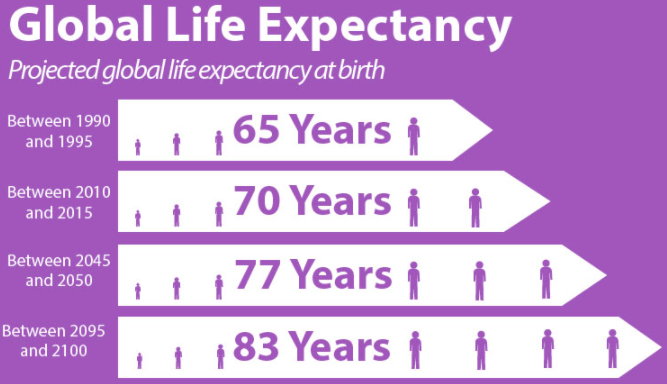
\includegraphics[width=.9\columnwidth]{expectancy.png}}
					\caption{\small Source: \textit{World Population Prospects: 2017 Revision.}}
					\label{esperanza}
				\end{figure}

				\begin{figure}[h]
				\vspace{-0.4cm}
					\centering
					\fbox{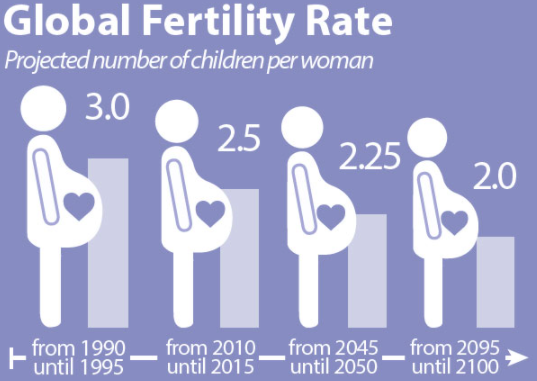
\includegraphics[width=.9\columnwidth]{fertility.png}}
					\caption{\small Source: \textit{World Population Prospects: 2017 Revision.} United Nations Department of Economic and Social Affairs, Population Division.}
					\label{fertilidad}
				\end{figure}
				The evolution of the age structure of the population allows a better understanding of aging:
				\begin{figure}[h]
					\centering
					\fbox{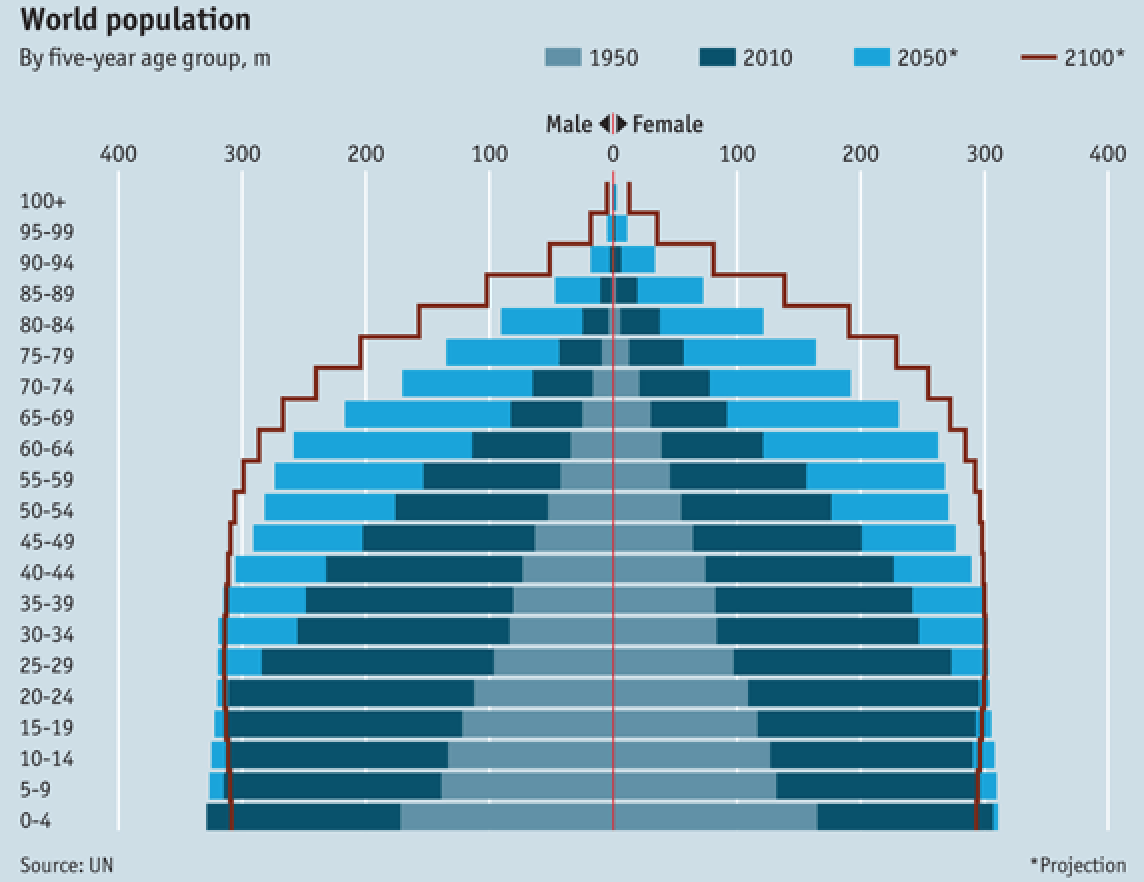
\includegraphics[width=.89\columnwidth]{piramide.png}}
					\caption{\small Worldwide population structure. Source: \textit{ONU.}}
					\label{piramide}
					\end{figure}
					\vspace{-0.4cm}
					A 47\% increasing in worldwide population is expected for the next 80 years.
				%Lorem ipsum dolor sit amet, consectetur adipiscing elit, sed do eiusmod tempor incididunt ut labore et dolore magna aliqua. Ut enim ad minim veniam, quis nostrud exercitation ullamco laboris nisi ut aliquip ex ea commodo consequat. Duis aute irure dolor in reprehenderit in voluptate velit esse cillum dolore eu fugiat nulla pariatur. 
				\begin{figure}[h]
					\centering
					\fbox{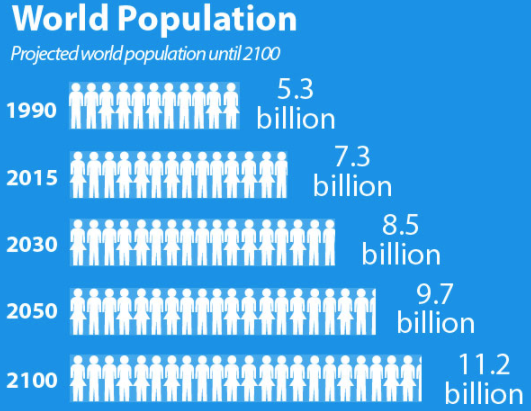
\includegraphics[width=.9\columnwidth]{population.png}}
					\caption{\small Source: \textit{World Population Prospects: 2017 Revision.} United Nations Department of Economic and Social Affairs, Population Division.}
					\label{poblacion}
				\end{figure}
				\vspace{-0.9cm}
				%Lorem ipsum dolor sit amet, consectetur adipiscing elit, sed do eiusmod tempor incididunt ut labore et dolore magna aliqua.
			\end{multicols}
		\end{block}

\vspace{-0.5cm}
%%%%%%%%%%%%%%%%%%% MODELOS DE MORTALIDAD  %%%%%%%%%%%%%%%%%%%%
		\begin{block}{Stochastic Mortality Modelling for Spanish Population with StMoMo}\vspace{-0.5cm}
			\setlength{\parindent}{1.2em}
			\setlength{\parskip}{1ex}
			The R package StMoMo \textcolor{blue}{(Villegas et. al., 2017)} is used to project the mortality rate according to age, sex and time for the spanish population.
			%Lorem ipsum dolor sit amet, consectetur adipiscing elit, sed do eiusmod tempor incididunt ut labore et dolore magna aliqua. Ut enim ad minim veniam, quis nostrud exercitation ullamco laboris.
\vspace{-1cm}     %%%%%%%%%%%%%%% CARACTERÍSTICAS  %%%%%%%%%%%%%%%%%%%

			\begin{columns}[t]
			\column{.47\columnwidth} %%%%%%%%%% MOST IMPORTANT MODELS  %%%%%%%
				\begin{block}{Models Comparison}
				%\vspace{0cm}
				\setlength{\parindent}{1.2em}
				\setlength{\parskip}{1ex}\vspace{-0.75cm}
					\noindent Based on two criteria:\vspace{-0.3cm} 
					\begin{enumerate}
						\item Quantitative Criteria:
						\begin{enumerate}
							\item[$\Rightarrow$] Bayes Information Criteria (BIC).
							\item[$\Rightarrow$] Incomplete. Doesn't provide all the information.
						\end{enumerate}
						\item Qualitative Criteria:
						\begin{enumerate}
							\item[$\Rightarrow$] Transparency and reasonable forecasting.
							\item[$\Rightarrow$] Age and period robustness.
							\item[$\Rightarrow$] Biologically reasonable.				
						\end{enumerate}
						%\item Maecenas tempus spectrae.
						%\item Quisque rutrum. Aenean imperdiet.
					\end{enumerate}
				\end{block}\vspace{-1cm}
				\begin{block}{Most Important Models}\vspace{-0.5cm}
				\textit{Lee-Carter}, (1992); \textit{Renshaw-Haberman}, (2006); \textit{Age-Period-Cohort} (APC); \textit{Cairns-Blake-Dowd}, (2006); \textit{Cairns et. al.}, (2007a y 2007b),...
					%~ \begin{flushright}
						%~ \includegraphics[height=10ex]{python_logo}
						%~ \includegraphics[height=10ex]{scipy_logo}
					%~ \end{flushright}
				\end{block}
				\column{.47\columnwidth} %%%%%%%%%% NEED OF THE MODELS  %%%%%%%
				\begin{block}{The Need of Mortality Models}\vspace{-0.5cm} 
					\begin{itemize}
						\item With reliable data, the underlying process is driven by a stochastic process.
						\item Mortality evolution uncertainty.
						\item Better \textbf{longevity risk management}.
						\item Risk reserve setting.
						\item Design of \textit{insurance-life contracts with integrated options.}
						\item Pricing and hedging of assets ​​linked to mortality.
						\item Improving strategies for pension funds and policymakers.																		%\begin{itemize}
						%	\item Quis autem vel eum iure reprehenderit qui in ea.
						%\end{itemize}
						%\begin{itemize}
							%\item Lor separat existentie es un myth. 
						%\end{itemize}
					\end{itemize}
				\end{block}
			\end{columns}
			\vspace{-1cm}
			\begin{figure}[h]
				\centering
				%\begin{columns}[t]
				%\column{.33\columnwidth}
				     %\fbox{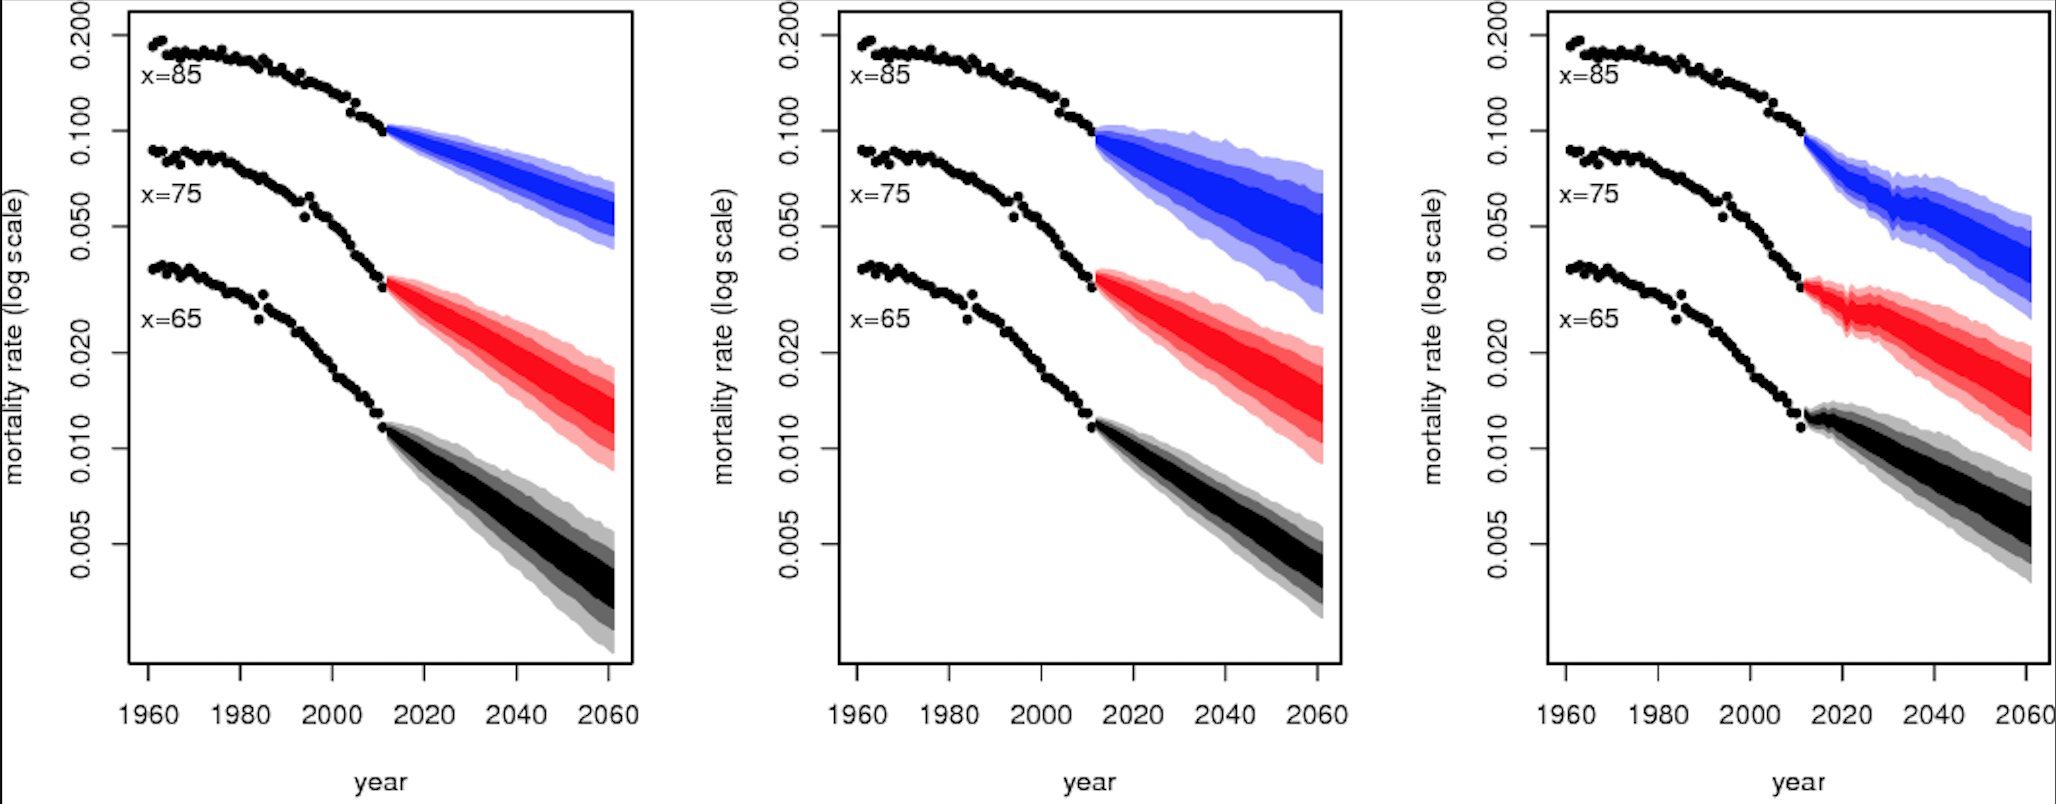
\includegraphics[width=.88\columnwidth]{modelos.png}}
					\fbox{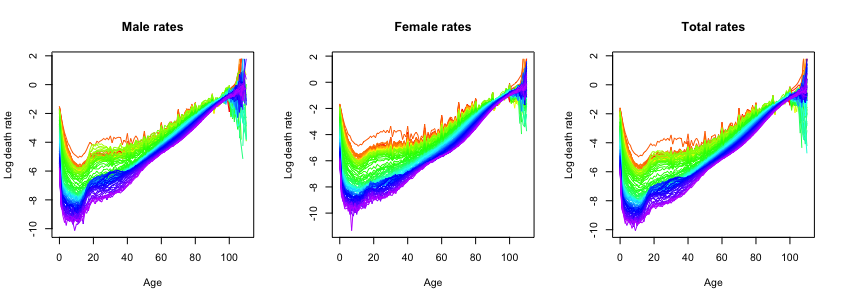
\includegraphics[width=.9\columnwidth]{mort.png}}
					\caption{\small  Logarithm pattern of mortality rates according to age and time for the Spanish population. Several behaviors are shown, respectively, for men, women, and total population. For the Lee-Carter model (without the logarithmic transformation) the \textttt{\textbf{R}} function \textit{``lca''} can be used, also being applied separately between men, women and the total population and considering a maximum age of 100 years.}
					%\caption{\small Gr\'aficos de dispersi\'on para las tasas de mortalidad $qxt$ en las edades $x = 65$ (abanico inferior), $x = 75$ (abanico medio) y $x = 85$ (abanico superior) de tres modelos ajustados a la poblaci\'on masculina de Inglaterra y Gales para las edades de 55-89 y per\'iodo 1961-2011. Los puntos muestran tasas hist\'oricas de mortalidad para 1961-2011. Las sombras en el abanico representan los intervalos de predicci\'on al 50\%, 80\% y 95\%.}
					%\label{modelos}
				%\column{.32\columnwidth}
				%	\includegraphics[width=0.9\columnwidth]{gr\'afico_2.png}
				%	\caption{\small }
				%	\label{fig_background-removal}
				%\column{.32\columnwidth}
				%	\includegraphics[width=0.9\columnwidth]{gr\'afico_3.png}
				%	\caption{\small }
				%	\label{fig_energy-calibration}
			%	\end{columns}
			\end{figure}
\vspace{-0.2cm}
			%Lorem ipsum dolor sit amet, consectetur adipiscing elit, sed do eiusmod tempor incididunt ut labore.
		\end{block}
		
%\vspace{-0.5cm}  %%%%%%%%%%%%%%%%%%%%%%%%%%%%%%%%%%%%%%%%%%%%%%%	
%		\begin{block}{ABCEFDAGADFA}
%			\setlength{\parindent}{1.2em}
%			\setlength{\parskip}{1ex}

%			Using the Python programming language we have written a program (licensed under GPL, available for download at \cite{emcd_tool}) for the comfortable treatment of EELS spectra for determination of EMCD signals.
%		\end{block}
%%%%%%%%%%%%%%%%%%%%%%%%%%%%%%%%%%%%%%%%%%%%%%%	
	
	\column{.515\textwidth}\vspace{-1.5cm}   %%%%%%% LAS PENSIONES EN ESPAÑA %%%%%%%%%%%
		
		\begin{block}{European Fertility Rates}
		Fertility rates in Europe are decreasing at all levels: by country and region. The spanish case is particularly severe.
					\begin{figure}[h]
						\fbox{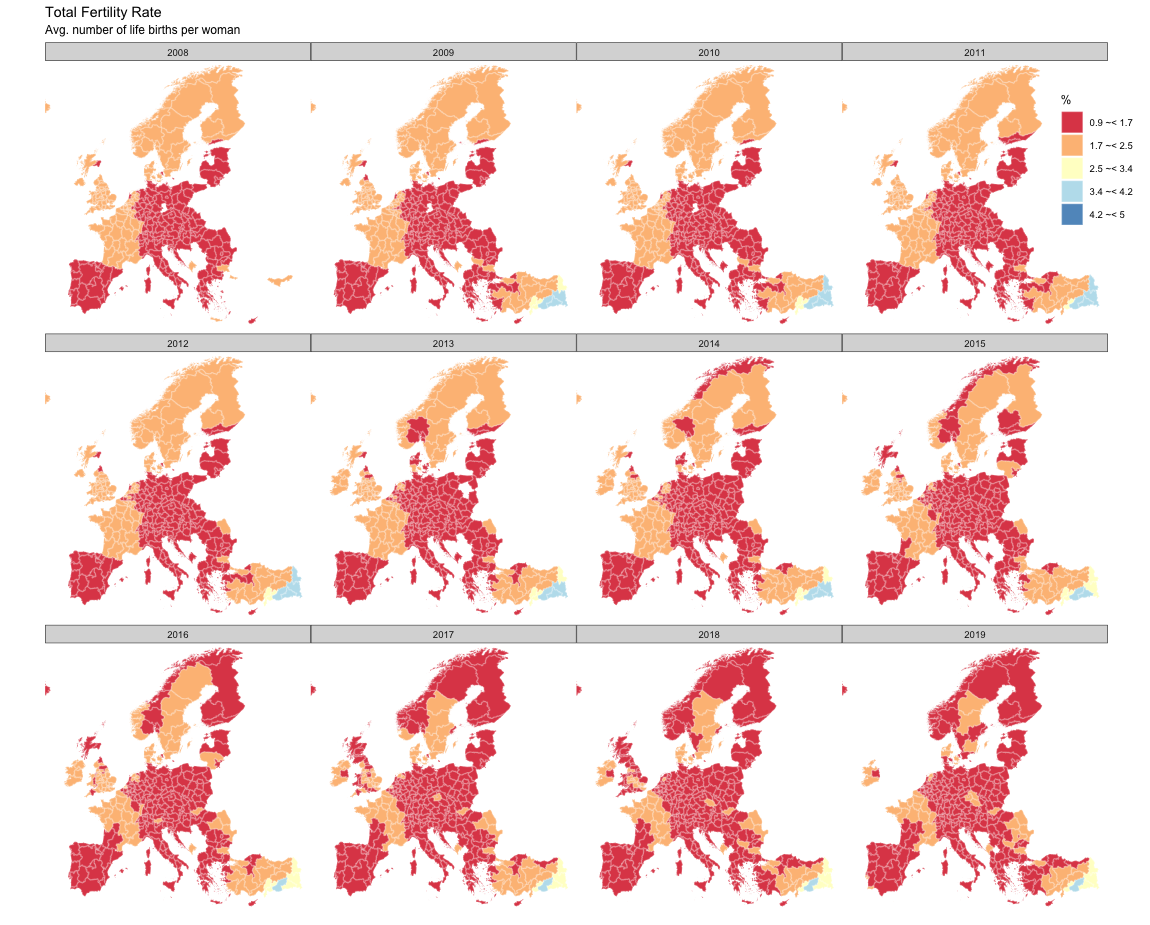
\includegraphics[width=.95\columnwidth]{fert_eu.png}}
						\caption{\small Total Fertilty Rate (average number of births per woman NUTS-3 level. \textit{Source: EUROSTAT.}}
						\label{pension1}
					\end{figure}\vspace{-0.5cm}
			% \begin{columns}[t]
				% \column{.45\columnwidth}
					% \begin{figure}[h]
						% \includegraphics[width=.6\columnwidth]{gr\'afico_4.png}
						% \caption{\small Lorem ipsum dolor sit amet, consectetuer adipiscing elit. Aenean commodo ligula eget dolor. Aenean massa. Cum sociis natoque penatibus et magnis dis parturient montes.}
						% \label{emcd_twinview}
					% \end{figure}
				% \column{.45\columnwidth}
					% \begin{figure}[h]
						% \includegraphics[width=.6\columnwidth]{gr\'afico_5.png}
						% \caption{\small Lorem ipsum dolor sit amet, consectetuer adipiscing elit. Aenean commodo ligula eget dolor. Aenean massa.}
						% \label{emcd_70}
					% \end{figure}
			% \end{columns}
			% \begin{multicols}{2}
			%		\begin{itemize}
			%			\item El gasto en pensiones aument\'o un 7\% en enero, hasta la cifra de 9.535 millones de \euro.
			%			\item Los efectos del envejecimiento deben contrarrestarse mediante un conjunto amplio de pol\'iticas: natalidad, conciliaci\'on, inmigraci\'on, reformas estructurales,...
			%			\item En Espa\~na, las condiciones demogr\'aficas del pasado y favorables para el sistema, no se repetir\'an en el futuro, por lo que se debe asegurar la sostenibilidad del mismo.
			%			\item En nuestro pa\'is, el importe medio de la pensi\'on es de 938 \euro\ y de la pensi\'on de jubilaci\'on de 1.085 \euro.						
			%			\item Application of a filter reduces noise considerably, \textbf{but} gives rise to "background oscillations" (see fig. \ref{emcd_70}).
			%			\item Increasing the kernel size of the filter results in stronger reduction of noise, \textbf{but} broadens features and decreases the height of the \ce{L23} edges.
			%		\end{itemize}
			%	\end{multicols}
			%	\vspace{-2.5cm}
			%\	begin{columns}[t]
			%	\column{.48\columnwidth}
			\begin{figure}[ht]
				\begin{minipage}[b]{.5\textwidth}
				\centering
				\fbox{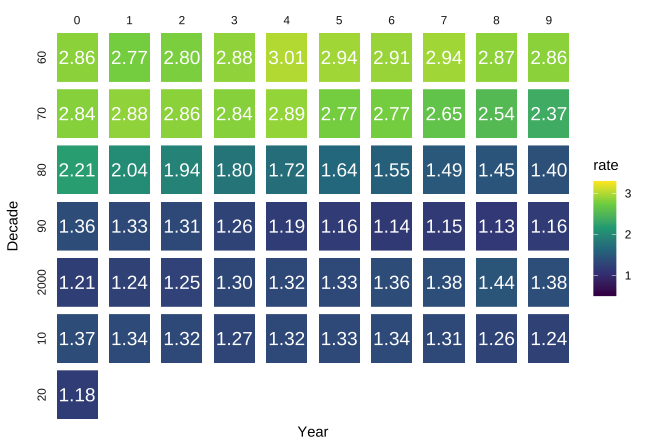
\includegraphics[width=1\textwidth]{fert_rate_sp2.png}}
				\caption{Spanish Fertility Rate Evolution 1960-2020. \textit{Source: Eurostat}}
				\end{minipage}
				\hfill
				\begin{minipage}[b]{.48\textwidth}
				\centering
				\fbox{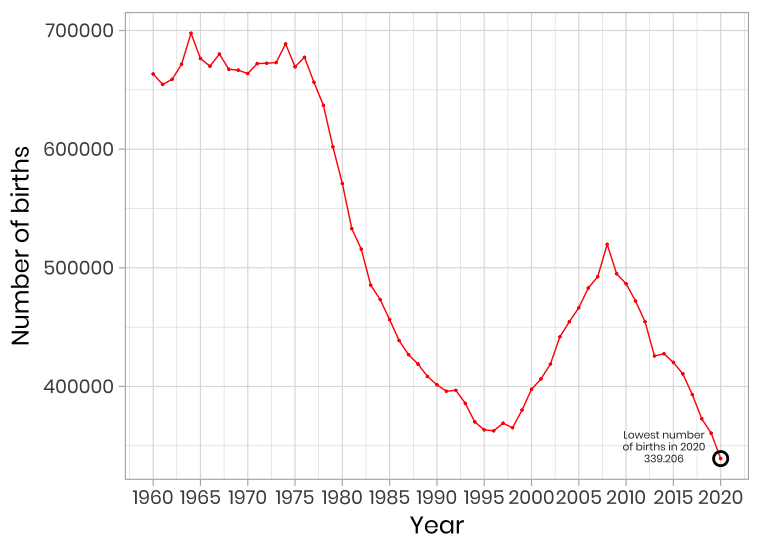
\includegraphics[width=0.99\textwidth]{births_sp2.png}}
				\caption{\small Number of births is Spain 1960-2020. \textit{Source: INE}}
				\end{minipage}
			\end{figure}
		%\end{block}
					%\begin{figure}[h]
					%	\fbox{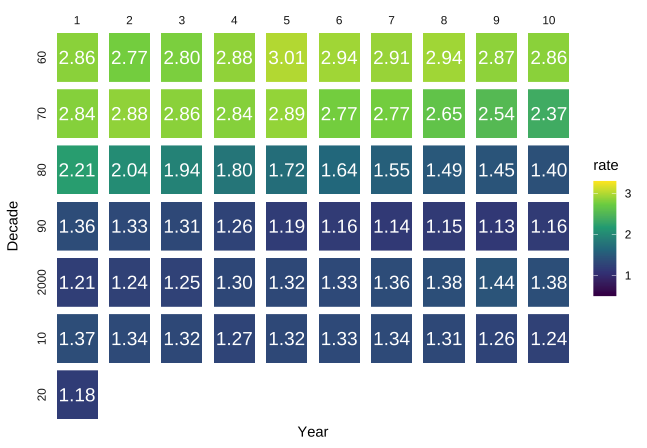
\includegraphics[width=0.505\columnwidth]{fert_rate_sp.png}}\fbox{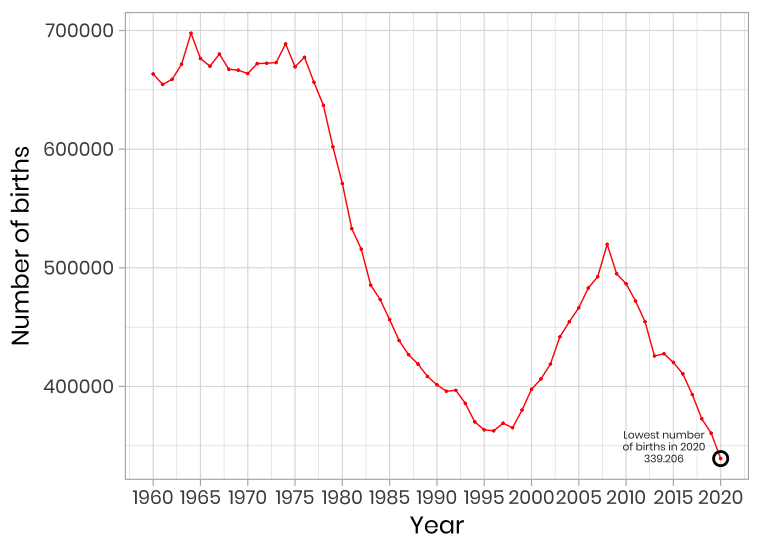
\includegraphics[width=0.48\columnwidth]{births_sp2.png}}
					%	\caption{\small Spanish Fertility Rate Evolution 1960-2020. \textit{Source: Eurostat}\caption{\small Number of births is Spain 1960-2020. \textit{Source: INE}}
						%\label{fertratevol}
					%\end{figure}\vspace{-2cm}
					%\begin{figure}[h]
						%\label{births}
					%\end{figure}
					\vspace{-0.5cm}
					\begin{minipage}{.98\columnwidth}
					\begin{block}{Fitting and Projection of the ’bayesTFR’ Model for the Spanish Population}
					The model proposed by \textcolor{blue}{\v{S}ev\v{c}{\'\i}kov\'{a} et al. (2011)} uses 5-year estimates of the TFR (Total Fertility Rate) from several periods and based on the observation that the evolution of  TFR includes three broad phases: Phase I: a pre- transitional high fertility phase; Phase II: the transition to fertility in which the TFR decreases from high fertility levels to or below the replacement fertility level and Phase III, where after the low fertility transition, which includes recovery of fertility below replacement towards replacement fertility and oscillations around fertility at that same level.
					%\column{.48\columnwidth}
					\begin{figure}[h]
\begin{minipage}[b]{.5\textwidth}
\centering
\fbox{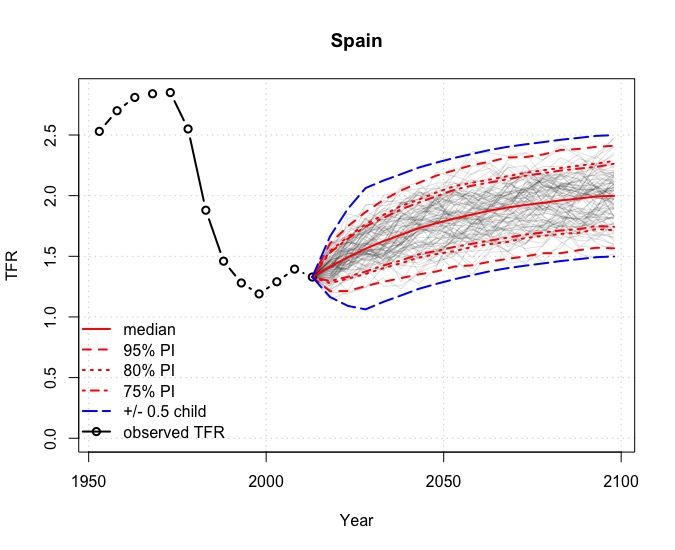
\includegraphics[width=0.94\textwidth]{bayesTFR01.jpeg}}
\caption{Spanish Fertility Rate Projections. \textit{}}
\end{minipage}
\hfill
\begin{minipage}[b]{.48\textwidth}
\centering
\hspace{-1.25cm}\fbox{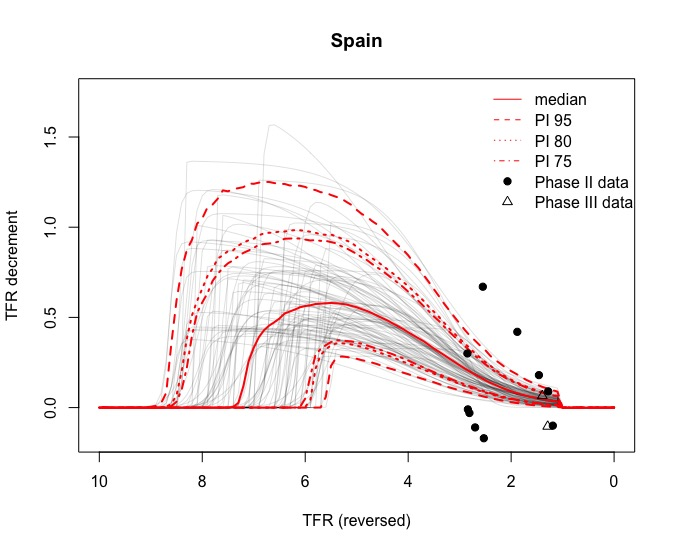
\includegraphics[width=0.98\textwidth]{bayesTFR02.jpeg}}
\caption{\small Spain (hierarchical) mean of the decline curve. \textit{}}
\end{minipage}
\end{figure}
\end{block}
\end{minipage}
\vspace{-1.75cm}
					%\begin{figure}[h]
						%\fbox{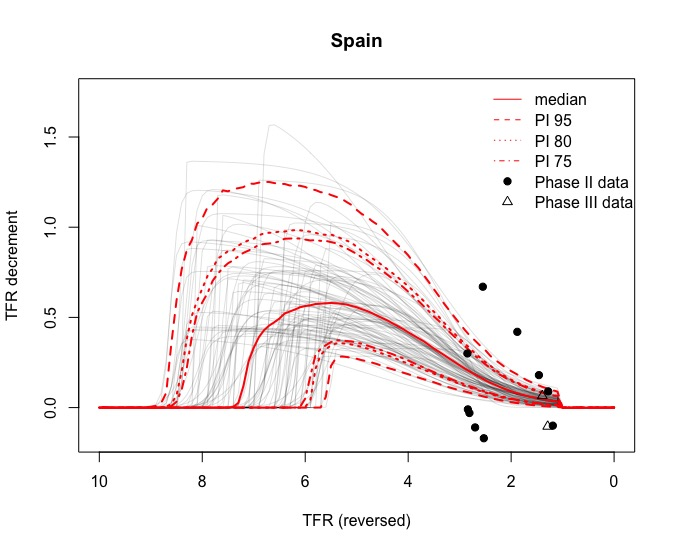
\includegraphics[width=0.5\columnwidth]{bayesTFR02.jpeg}}
						%\caption{\small Instrumentos de ahorro menos preferidos.}
						%\label{ahorro1}
					%\end{figure}
			%\end{columns}
		\end{block}
		
		\vspace{-0.5cm}
%%%%%%%%%%%%%%%%  PRINCIPALES RESULTADOS %%%%%%%%%%%%%%%%%%%%%%%%
%\begin{block}{La Hipoteca Inversa como Complemento a la Pensi\'on}\vspace{-0.8cm}
	%		\begin{multicols}{2}
	%			%\column{.48\columnwidth}
	%				\setlength{\parindent}{1.2em}	
	%				\setlength{\parskip}{1ex}
	%			\begin{itemize}
	%				%\item En la b\'usqueda de nuevas f\'ormulas de ahorro y previsi\'on, surge la figura de la hipoteca inversa.
	%				\item Poco conocida y  contratada en nuestro pa\'is, no tiene excesiva aceptaci\'on por diversos motivos:
	%					\begin{enumerate}
	%						\item[$\Rightarrow$] Caracter\'isticas del sector inmobiliario espa\~nol.
	%						\item[$\Rightarrow$] Dif\'icil de entender para los ancianos.
	%						\item[$\Rightarrow$] Implicaciones emocionales (apego a la vivienda).
	%						\item[$\Rightarrow$] Normalmente para inmuebles de alto valor.					
	%					\end{enumerate}
	%				\item A cambio de la propiedad de la vivienda, se recibe una especie de pensi\'on privada como alternativa o complemento a la pensi\'on p\'ublica.
	%				\item Al poner como garant\'ia esa vivienda de la que es titular, el prestatario recibe dinero mediante disposiciones peri\'odicas o en una sola entrega.
	%				\item Goza de beneficios fiscales y financieros.
	%				\end{itemize}
	%				\vspace{-1cm}		
	%				\begin{table}[h] 
	%					\begin{tabular}{|c|c|c|c|c|c|}
	%						\hline
	%						Edad & \multicolumn{4}{|c|}{\bfseries Valor tasaci\'on vivienda} & Duraci\'on\\ \cline{2-5}
	%						 & 100.000 & 200.000 & 300.000 & 400.000 & de la renta \\ \hline
	%						 \rowcolor[gray]{0.8}70 & 157,96 & 325,76 & 493,75 & 662,36 & 20 \\ \hline
	%						 75 & 218,49 & 447,06 & 676,30 & 905,78 & 17 \\ \hline
	%						 \rowcolor[gray]{0.8}80 & 306,36 & 623,22 & 941,39 & 1.259,29 & 14 \\ \hline
	%						 85 & 434,59 & 882,68 & 1.331,48 & 1.780,90 & 11 \\ \hline
	%						 \rowcolor[gray]{0.8}90 & 582,20 & 1.178,64 & 1.776,84 & 2.374,69 & 9 \\ \hline
	%						 %70 & 157,96 & 325,76 & 493,75 & 662,36 & 20 \\ \hline
	%					\end{tabular}
	%					\caption{Simulaciones de rentas mensuales temporales en funci\'on de la edad y del valor de la vivienda.}
	%					\label{renta}
	%				\end{table}
%\vspace{-0.3cm}					
	%		\end{multicols}
	%		\vspace{-0.6cm}
			\noindent
			\begin{minipage}{.999\columnwidth}
				\begin{block}{Conclusions}\vspace{-0.6cm}
				A three-parameter model can capture most of the variation in the fertility and mortality patterns observed. Models with more parameters, for most of the purposes, they are not necessary, and they may experience difficulties adapting such models to a small number of data.
					%\begin{multicols}{2}
					%	\setlength{\parindent}{1.2em}	
					%	\setlength{\parskip}{1ex}
					%	\begin{itemize}
					%		\item Afrontamos un problema demogr\'afico de envejecimiento paulatino e incremento de las expectativas de vida.
					%		\item Se hace necesario minimizar el riesgo de longevidad mediante modelos de mortalidad fiables.
					%		\item Fundamental la planificaci\'on financiera: 
					%			\begin{enumerate}
					%				\item[$\Rightarrow$] \textbf{Estatal:} cambios en el sistema para garantizar las pensiones.
					%				\item[$\Rightarrow$] \textbf{Individual:} con productos alternativos que complementen la pensi\'on.
					%			\end{enumerate}
					%		\item La hipoteca inversa puede ser una opci\'on interesante que garantice liquidez para necesidades de consumo y m\'edicas o asistenciales durante la vejez.
					%	\end{itemize}
				%	\end{multicols}
				%	\vspace{-0.5cm}
				\end{block}
			\end{minipage}
		%\end{block}
		\noindent
		
		\vspace{-0.5cm}
		
			\begin{block}{Extract of Most Relevant References}\vspace{-0.4cm}
				\begin{itemize}
				%\item[1.] Ehrlich, P.: \textbf{The Population Bomb}, Ballantines Books 1st ed. (1968).
				%\item[1.] Tapinos, G. P.: \textbf{El\'ements de D\'emographie}, A. Colin, (1985).
				%\item[1.] Lee, R. D. and Carter, L. R. (1992): \textbf{Modeling and Forecasting U. S. Mortality}, Journal of the American Statistical Association, 87, 419, Sept.
				\item[1.] Villegas, A., Kaishev, V., Milosovich, P. (2017): \textbf{StMoMo: An R Package for Stochastic Mortality Modeling}.
				\item[2.] \v{S}ev\v{c}{\'\i}kov\'{a}, H., Alkema, L. and Raftery, A. E. (2011): \textbf{bayesTFR: An R Package for Probabilistic Projections of the Total Fertility Rate}, Journal of Statistical Software, 43, 1, 1-29 \texttt{https://www.jstatsoft.org/v43/i01/}
				%\item[6.] F.E. Wagner et al., \textbf{Electronic Structure and Properties of Hydrogen in Metals}, (1983), p. 581-595
				%\item[8.] [...]
				%\item[9.] [...]
				%\item[10.] [...]
				\end{itemize}\vspace{-0.3cm}
				\end{block}
			
	\end{columns}
\end{frame}
\end{document}
